\begin{figure}[h]
  \centering
  \begin{tabular}{ c p{0.2cm} c p{0.2cm} p{3.5cm} }
    %\centering
    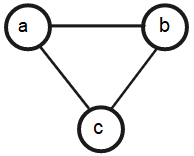
\includegraphics[width=2.3cm]{./img/trianguloabc.png} && 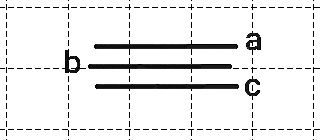
\includegraphics[width=3.5cm]{./img/b0epgTransparenciaGrade2.png} & &
    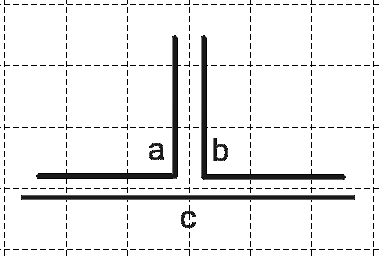
\includegraphics[width=3.5cm]{./img/b1EpgTransparenteGrade2.png}
    \\
    \footnotesize %\centering 
    (a) The  graph $C_3$ && \footnotesize(b) $B_0$-EPG representation of $C_3$ && (c) $B_1$-EPG representation of $C_3$\\
%& &  \\ \centering
%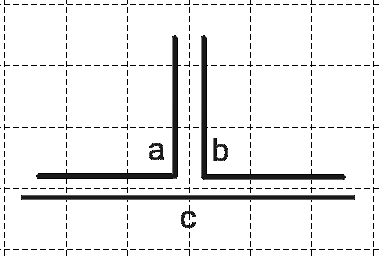
\includegraphics[width=3.5cm]{./img/b1EpgTransparenteGrade2.png} %b1epgtriangulo
 %    & 
  %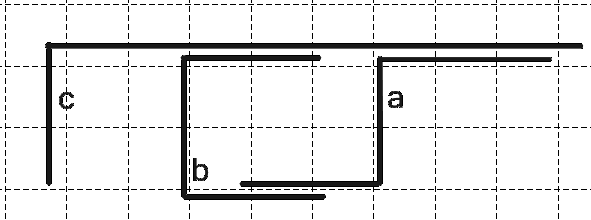
\includegraphics[width=5cm]{./img/b2epgTransparenciaGrade2.png}\\
%   \footnotesize \centering (c) $B_1$-EPG representation of $C_3$  &  \footnotesize  (d) $B_2$-EPG representation of $C_3$ \\
  \end{tabular}

 \caption{The  graph $ C_3 $  and  representations without bends and with 1 bend} \label{fig:trianguloepgRepresentacao}
\end{figure}